\documentclass[twoside]{article}

\usepackage[sc]{mathpazo} % Use the Palatino font
\usepackage[T1]{fontenc} % Use 8-bit encoding that has 256 glyphs
\linespread{1.05} % Line spacing - Palatino needs more space between lines
%\usepackage{microtype} % Slightly tweak font spacing for aesthetics

\usepackage[twoside,width=16cm,height=24cm,left=3cm]{geometry}
%\usepackage[hmarginratio=1:1,top=20mm,width=19cm,height=23cm,columnsep=15pt]{geometry} % Document margins
\usepackage{multicol} % Used for the two-column layout of the document
\usepackage[hang, small,labelfont=bf,up,textfont=it,up]{caption} % Custom captions under/above floats in tables or figures
\usepackage{booktabs} % Horizontal rules in tables
\usepackage{float} % Required for tables and figures in the multi-column environment - they need to be placed in specific locations with the [H] (e.g. \begin{table}[H])
\usepackage{hyperref} % For hyperlinks in the PDF

%----------- Agregados para el caso de ustedes -------------------------------
\usepackage[spanish]{babel}% idioma castellano
\usepackage[utf8]{inputenc}% esto es para poder poner los tildes directamente. Puede que cambie de versión a versión de sistema operativos (más información en http://www.aq.upm.es/Departamentos/Fisica/agmartin/webpublico/latex/FAQ-CervanTeX/FAQ-CervanTeX-6.html )
\usepackage{graphicx} % para insertar figuras
\usepackage{subfigure} % para insertar figuras dentro de figuras
\usepackage{times} % plataforma
\usepackage{amsmath} % --para ecuaciones y algunos símbolos 
\usepackage{soul}
% ---------------------- -----------------------------------------------------

\usepackage{lettrine} % The lettrine is the first enlarged letter at the beginning of the text
\usepackage{paralist} % Used for the compactitem environment which makes bullet points with less space between them

\usepackage{abstract} % Allows abstract customization
\renewcommand{\abstractnamefont}{\normalfont\bfseries} % Set the "Abstract" text to bold
\renewcommand{\abstracttextfont}{\normalfont\small\itshape} % Set the abstract itself to small italic text
\addto\captionsspanish{ % Modifica algunos nombres cambiandolos por los definidos a continuacion
        \def\contentsname{\'Indice}%
        \def\bibname{Referencias}%
        \def\tablename{Tabla}%
        \def\abstractname{Resumen}
        }
\usepackage[usenames,dvipsnames,svgnames,table]{xcolor}
%\usepackage{natbib}
%\usepackage[usenames]{color}
\usepackage{graphicx}
\usepackage[spanish]{babel}
\usepackage{amsmath}
\usepackage{float}
\usepackage{dsfont}
\usepackage{textcomp}
\usepackage{soul}
\usepackage{fancyhdr}
\usepackage{titlesec} % Allows customization of titles
\usepackage{fancyhdr} % Headers and footers
\usepackage[spanish]{babel}
\usepackage{amsmath}
\usepackage{hyperref}


\pagestyle{fancy} % All pages have headers and footers
\fancyhead{} % Blank out the default header
\fancyfoot{} % Blank out the default footer
\fancyhead[C]{Laboratorio  $\bullet$ 16 de febrero de 2018} % Custom header text
\fancyfoot[RO,LE]{\thepage} % Custom footer text




%----------------------------------------------------------------------------------------
%	TITLE SECTION
%----------------------------------------------------------------------------------------

\title{\vspace{-15mm}\fontsize{24pt}{10pt}\selectfont\textbf{Radiación gamma: estudio de fuentes radiactivas}} % Article title

\author{
\large
\textsc{Leandro Pezzente, Lucía Evangelista Gallo}\\[2mm] %  Autores. Van entre comas y en orden alfabético
\normalsize Laboratorio 5, FCEyN, UBA \\ % Your institution. Filiación
%\small \href{mailto:perez@gmail.com}{perez@gmail.com} % Your email address
\vspace{-5mm}
}
\date{}

%----------------------------------------------------------------------------------------


\begin{document}

\maketitle % Insert title

\thispagestyle{fancy} % All pages have headers and footers

%----------------------------------------------------------------------------------------
%	ABSTRACT
%----------------------------------------------------------------------------------------

\begin{abstract*}
En este trabajo se presentan y comentan los resultados de las experiencias realizadas para estudiar fenómenos relacionados con la radiación gamma. Se trabajó con cuatro fuentes, $^{137}$Cs, $^{22}$Na, $^{207}$Bi y $^{133}$Ba; unicamente con la fuente $^{137}$Cs fue posible observar un espectro donde la meseta Compton era distinguible. El espectro se modeló utilizando una función que buscaba combinar los perfiles de los fenómenos presentes. 

La segunda parte de la experiencia consistió en interponer láminas de cobre entre el detector y la fuente, al fin de estudiar la atenuación que sufre la radiación al interactuar con materia. Se verificó la hipótesis de que la atenuación era de tipo exponencial y se encontró el coeficiente de atenuación lineal, $\mu_l = (0.8168 \pm 0.0002)$cm$^{-1}$.

\end{abstract*}

%----------------------------------------------------------------------------------------
%	ARTICLE CONTENTS
%----------------------------------------------------------------------------------------

\begin{multicols}{2} % Two-column layout throughout the main article text


\section*{\underline{Introducción}}
\noindent Cuando se quiere estudiar la interacción de la  radiación gamma con la materia, es importante tener en cuenta dos factores clave: en primer lugar, un rayo gamma debe interactuar con un detector para poder ser ``visto"; en segundo, la intensidad de la radiación es fuertemente dependiente con la distancia fuente -- instrumento.

La interacción de la radiación gamma con la materia se verifica a través de tres mecanismos dependientes del rango de energía en que se encuentren los fotones\cite{Nelson}: efecto fotoeléctrico para energías menores a la energía en reposo del electrón (511keV), dispersión Compton en la zona entre 511keV y 1022keV, y producción de pares positrón--electrón para energías mayores a 1022keV. %En la experiencia realizada no se verificó esta producción, pero sí se obtuvo un espectro que permitía apreciar el fenómeno Compton y el efecto fotoeléctrico. 

En relación a la dependencia espacial, se sabe que la atenuación de los rayos gamma es de tipo exponencial \cite{Nelson}:
\begin{equation}
    I = I_0  e^{-\mu _l L},
\end{equation}
donde $I$ es la intensidad transmitida por el material, $I_0$ la intensidad original, L el espesor del material y $\mu_l$ el coeficiente de atenuación (en cm$^{-1}$). Además, la relación entre el coeficiente de atenuación y la densidad del material es practicamente constante para todos los materiales.

\iffalse

La emisión de fotones gamma es, como ya se mencionó, un proceso aleatorio\cite{poisson}. A nivel microscópico, no es posible determinar ni la dirección ni el momento en que se producirá la emisión. Sin embargo, cuando se cuenta con una muestra macroscópica, esto es, un número mayor a 10$^{12}$ de átomos que decaen, se puede establecer el número promedio de decaimientos en una dada dirección. Los valores obtenidos estarán distribuidos alrededor de un valor medio <n>  y, para describir el proceso, se utiliza la distribución de Poisson:
\begin{equation}
    P_l (n) = \frac{l^n}{n!} e^{-l}, 
\end{equation}
con $n$ la variable aleatoria (número natural) y $l$ un parámetro característico de la distribución, tal que
\begin{equation}
    <n> = \sum [n*P_{\lambda}(n)] = l.
\end{equation}

\fi

En este trabajo se presentan y comentan los resultados de experimentos diseñados para estudiar los fenómenos brevemente descritos en esta sección.


\section*{\underline{Desarrollo experimental}}

\iffalse

\section*{\underline{Equipamiento y Método de Detección  }}

///////////////////////////////////
\fi

La configuración base que se utilizó durante los experimentos fue la siguiente (Fig. \ref{experimental}): en una jaula hecha con ladrillos de plomo, se colocaron las fuentes y uno de los extremos de un \hl{fotomultiplicador (PMT) de tipo NaI(TI)} (\textcolor{Blue}{un tubo detector compuesto por un cristal centellador NaI(Ti) acoplado a un fotomultiplicador (PMT)}). La jaula fue necesaria tanto para evitar que la radiación de las fuentes escapara al ambiente como para que la radiación exterior no influyera en las mediciones. Asimismo, como la atenuación del fenómeno con la distancia es considerable, las fuentes se colocaron lo más cercanas posible al detector. El PMT se alimentó con una fuente de alto voltaje seteado en 1.4kV (Canberra, modelo 30020) y estaba conectado a un amplificador (Canberra, modelo 2022).\textcolor{magenta}{Con un osciloscopio (MODELO, MARCA) se observó el cambio en el pulso al modificar los parámetros del amplificador. En particular, se buscó que la señal no saturara y que fuera lo más angosta posible \textcolor{cyan}{Es verdad esto???}. (\textcolor{Blue}{Los parametros de shaping del pulso depende de dos cosas , una el tiempo de decaimiento del centellador que anda alrededor de los 250 microsegundos y de la frecuencia de muestreo de la adquisidora, vos queres un ancho de shaping que sea la suficientemente angosto para compensar el tiempo de decaimiento del centellador pero no tan angosto como para que la adquisidora no te detecte todos los pulsos}) En base a esto, los valores fueron: coarse gain 3k, fine gain 80, shaping 8$\mu$ y polaridad positiva.}Los datos se adquirieron con una placa National Instruments USB -- 6210. Las fuentes utilizadas fueron $^{137}$Cs, $^{22}$Na, $^{207}$Bi y $^{133}$Ba. 

El PMT emite un pulso de tensión de amplitud proporcional a la energía incidente. Para conocer la relación de proporcionalidad, \hl{fue necesario calibrar el PMT.} (\textcolor{Blue}{como te decia en el mail, lo que calibras es el arreglo experimental entero, o mejor dicho calibras los pulsos detectados a la salida del amplificador con respecto a la energia de la muestra para los parametros de tu equipo experimental}) Para eso, se midió cada fuente, se hizo un histograma de voltajes registrados y se buscó el máximo. Luego, se graficaron los máximos medidos vs. los valores de energía tabulados, y se encontró la relación de proporcionalidad (ver sección siguiente). Para accionar el dispositivo, guardar y analizar los datos se utilizaron los software Matlab y GNU Octave.\hl{Se estableció para cada fuente un número de iteraciones en un rango de 300 a 900 de un segundo cada una, con una frecuencia de muestreo de 250kHz, y se tomó 0.5V como valor mínimo a partir del cual un dato se consideraba un pico.}(\textcolor{Blue}{Se estableció para cada medicion de datos un tiempo de adquisicion en un rango de 300 a 900 de un segundo , dependiendo de las caractiristicas de actividad de la fuente, configurando la adquisiodora NI-DAQ con una frecuencia de muestreo de 250kHz, y tomamdose un valor de canal de 0.5V para la cota maxima del ruido producido por diversos fenomenos en el tubo fotomultiplador.}) \textcolor{magenta}{Para determinar un valor a partir del cual un dato se consideraba un pico, se realizó una medición rápida de 0.002s con la muestra de $^{137}$Cs. A partir de las alturas de los picos, se decidió tomar un umbral de 0.5V. Teniendo en cuenta el nivel de emisividad de las fuentes con que se trabajó, el número de iteraciones varió entre 300 y 900, de un segundo cada una y con una frecuencia de muestreo de 250kHz, la máxima permitida por el dispositivo.}

En la segunda etapa de la experiencia, se fijó una distancia de $(12.95 \pm 0.01)$mm entre la fuente y el detector, y se fueron interponiendo láminas de cobre ($\rho = 10.4$g/cm$^3$) de distinto espesor (Tabla \ref{espesores}) en mediciones sucesivas.


\begin{figure}[H]
    \centering
    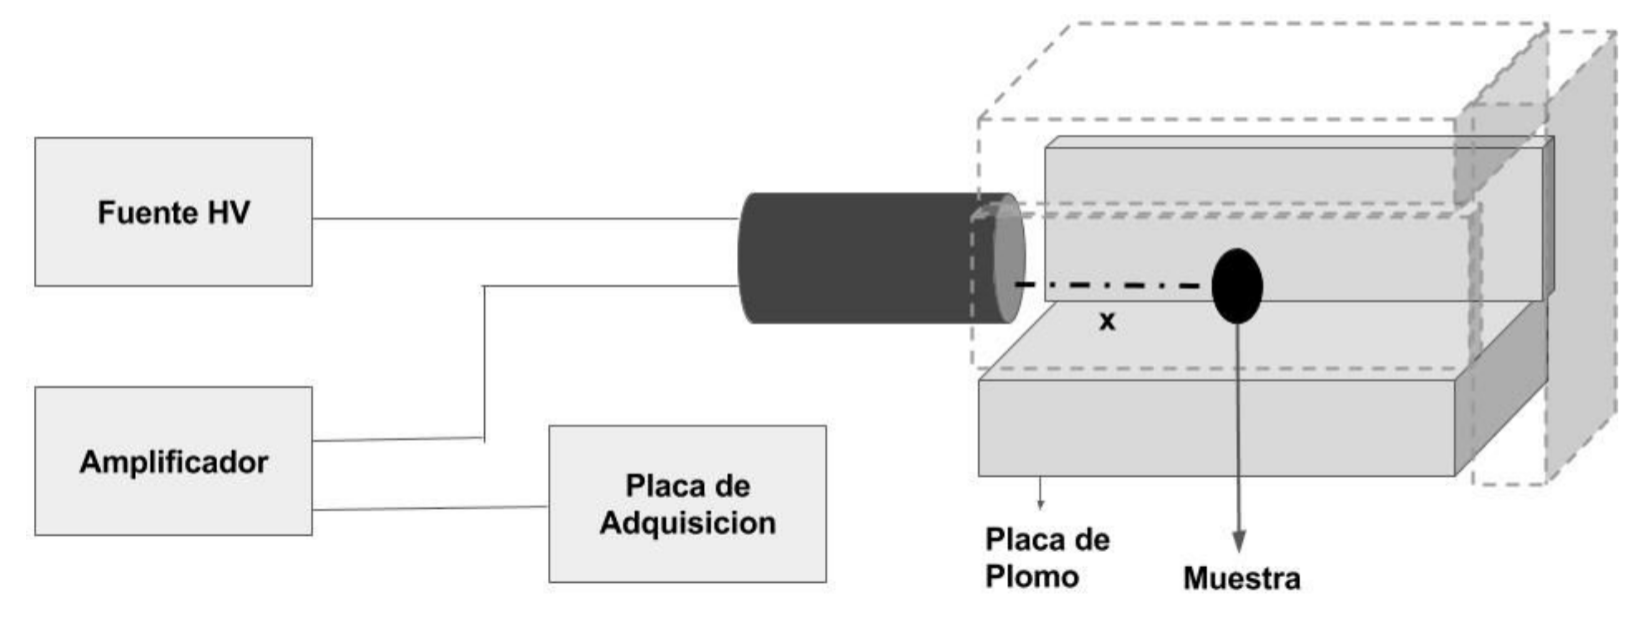
\includegraphics[scale=0.15]{ExpeNu.png}
    \caption{Configuración experimental base. Para realizar la segunda parte de la experiencia, se colocaron láminas de bronce entre el detector y la fuente. La distancia $x$ es ilustrativa; las muestras se colocaron lo más cercano posible al detector.}
    \label{experimental}
\end{figure}

\begin{table}[H]
    \centering
    \begin{tabular}{c|c}
         \hline
         Lámina & Espesor (mm) \\
         \hline 
         1 &  $(1.99 \pm 0.01)$mm\\\hline
         2 & $(4.00 \pm 0.01)$mm \\ \hline
         3 & $(1.99 \pm 0.01)$mm \\ \hline
         4 & $(1.98 \pm 0.01)$mm \\ \hline
         5 & $(1.99 \pm 0.01)$mm \\ \hline
         
    \end{tabular}
    \caption{Espesores de las láminas de cobre utilizadas.}
    \label{espesores}
\end{table}


%\section*{\underline{Interacción de radiación con materia}}
\iffalse
La interacción de la radiación gamma con la materia se da a través de tres mecanismos físicos básicos : efecto fotoeléctrico dominante en las energías menores a la energía en reposo del electrón ( 511 keV ), producción de pares positrón-electrón dominante para energías mayores a 1022 keV, y dispersión Compton , dominante en la zona intermedia entre 511 keV y 1022 keV. A la hora de hacer un análisis riguroso del interacción del los rayos gamma con la materia, es importante tener en cuenta los tres efectos, especialmente a la hora de analizar los efectos en la forma, ancho y localización de los picos de energía debidos a la interacción de la radiación gamma con el cristal centellador.

Un ejemplo de esto es la interacción de la radiación gamma con el cristal centellador que permite la detección de la radiación gamma. Esta interacción se da primariamente por efecto fotoeléctrico, especialmente a bajas energías donde este efecto es dominante. Los electrones en las capas interiores , mayoritariamente K y L , el átomo absorbe el fotón gamma al interactuar con el , transfiriendo esa energía a un electrón en las capas internas, el cual es dispersado al adquirir una energía mayor a la energía de enlace de la capa. El agujero dejado por el electrón dispersado es puede ser llenado mediante dos mecanismos, o bien puede capturar otro electrón de las capas mas internas o bien un electrón de las capas superiores puede decaer emitiendo un fotón en el rango de los rayos X, que usualmente es reabsorbido por los electrones circundantes, emitiendo excitando nuevos electrones, este fenómeno se denomina ``electrones Auger". El cristal centellador posee impurezas de materiales como el Tantalio (Tl) que absorbe los rayos X emitidos por el decaimiento de los electrones Auger y remite fotones en el rango del visible y ultravioleta, fenómeno conocido como "centellado". El numero de fotones en el visible es proporcional al numero de fotones de rayos X debidos a los electrones Auger, que a su vez es proporcional a la energía del fotón gamma.

La capacidad de la materia para interaccionar con los rayos gammas esta expresada por un coeficiente de atenuación lineal característico de dicha substancia. En particular el coeficiente de atenuación lineal tiene una dependencia funcional tanto con la densidad del material como con el numero atómico Z de la substancia, sin embargo, la forma funcional de la dependencia del coeficiente de atenuación lineal con Z depende fuertemente del cual de los tres tipos de interacción es la dominante para la escala de energía del foton gamma. Para las regiones en donde la interacción por dispersión Compton es dominante, este valor es aproximadamente constante.  
\fi


\section*{\underline{Resultados y análisis}}
En la Fig. \ref{histograma} se presenta el espectro de $^{137}$Cs. De las cuatro fuentes utilizadas, únicamente para el caso del cesio se puede apreciar la meseta Compton. Si bien de forma cualitativa, se puede diferenciar esta meseta entre 1V y 2V, seguido del fotopico entre 2V y 4V. Los puntos más elevados cerca de 1V podrían estar indicando presencia de back scattering. Las dos <<franjas>> de puntos se deben a que se utilizaron dos fuentes en simultáneo, una más activa que la otra. Los espectros del sodio y del bismuto presentaron dos picos. En la Fig. \ref{sodio}, correspondiente al espectro del sodio, se observa tanto la existencia de dos picos como la falta de definición de la meseta y borde Compton. Con respecto a esto último, la figura es representativa de lo que ocurrió con las fuentes de bismuto y de bario. Para mayor claridad en las figuras, se decidió no incluir los errores en algunas de ellas. Teniendo en cuenta la cantidad de procesos involucrados en el método de medición, se tomó un error del 10\%.

\begin{figure}[H]
    \centering
    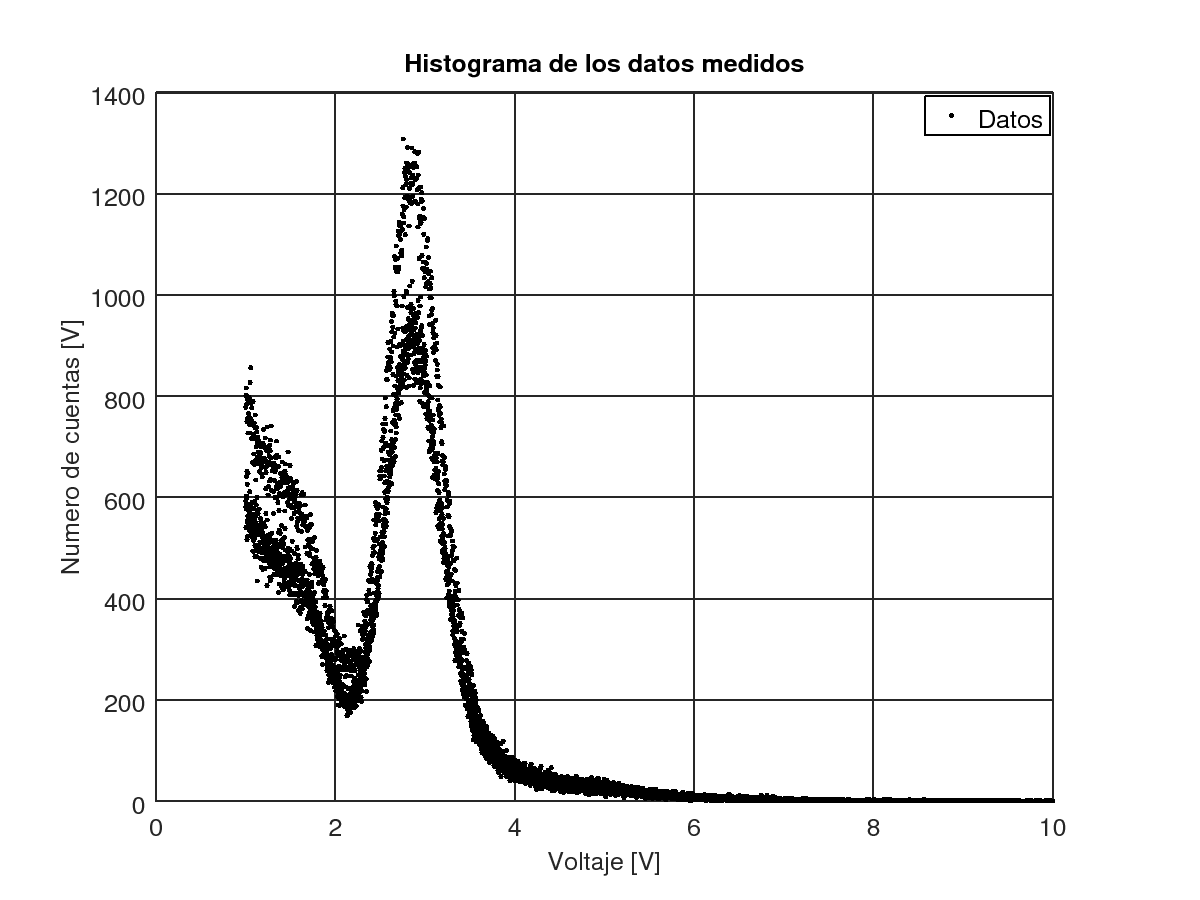
\includegraphics[scale=0.4]{espectro.png}
    \caption{Espectro del $^{137}$Cs. Las mediciones duraron 300 segundos.}
    \label{histograma}
\end{figure}

\begin{figure}[H]
    \centering
    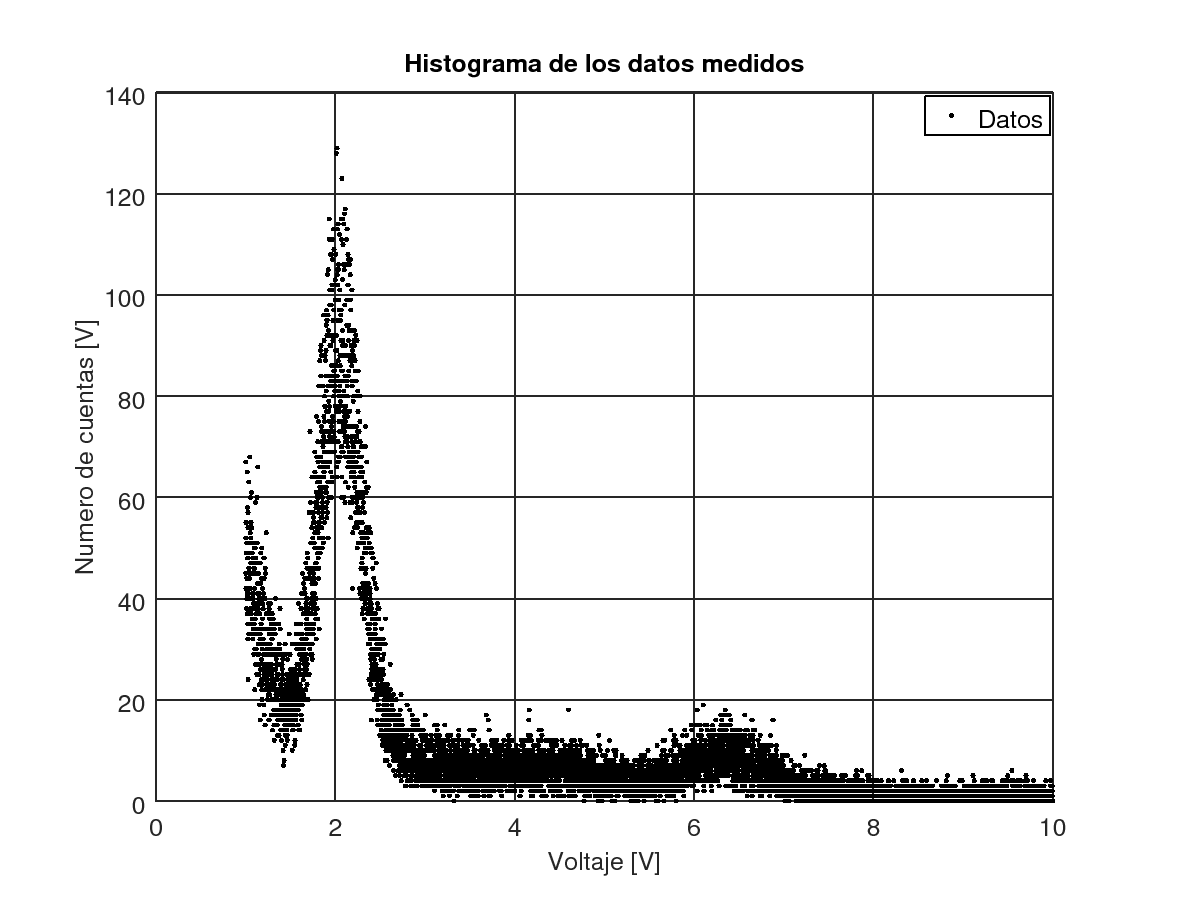
\includegraphics[scale=0.4]{sodio.png}
    \caption{Espectro del $^{22}$Na. Las mediciones duraron 900 segundos. El comportamiento de los datos en la región donde se esperaba observar la meseta Compton es representativa de lo ocurrido con $^{207}$Bi y $^{133}$Ba.}
    \label{sodio}
\end{figure}


Una vez obtenido el espectro de cada figura, se ajustaron los picos y se procedió a hacer la calibración. El ajuste se hizo modelando la mitad derecha del fotopico con una gaussiana,
\begin{equation}
    f(x) =  c + A e^{-\frac{(x - \mu)^2}{2\sigma^2}},
\end{equation}
con $c$ un offset, $A$ una constante de proporcionalidad, $\mu$ la media y $\sigma$ la varianza. Se hizo así para evitar que la presencia de la región Compton influyera en la determinación del máximo (evitar que éste se desplazara hacia la izquierda). Se eligió este procedimiento teniendo en cuenta que la función gaussiana es simétrica respecto de su eje y que, en la zona ajustada, ya no había presencia de efecto Compton. A partir de los ajustes se obtuvieron las posiciones de los picos. Luego, se graficaron estos datos $vs.$ los valores tabulados de energía correspondiente a cada fuente y cada pico (dos picos registrados para el $^{22}$Na y $^{207}$Bi) y se modeló con una lineal, obteniendo la siguiente relación: 
\begin{equation}
    y = 179.80 x + 125.97,
\end{equation}
donde $y$ serán los valores de energía, $x$ los de voltaje medido, y las unidades son keV. (\textcolor{Blue}{revisa de nuevo tu codigo en Octave, estoy 99.99\% seguro que estas tomando un linspace entre 1 y 10 Volts en vez de entre 0 y 10 Volts como tiene que ser, mira si te soy sincero, yo tuve que recalcular la curva de calibracion y me dio y = 161.82 x + 113.73  keV/Volt} )


\begin{figure}[H]
    \centering
    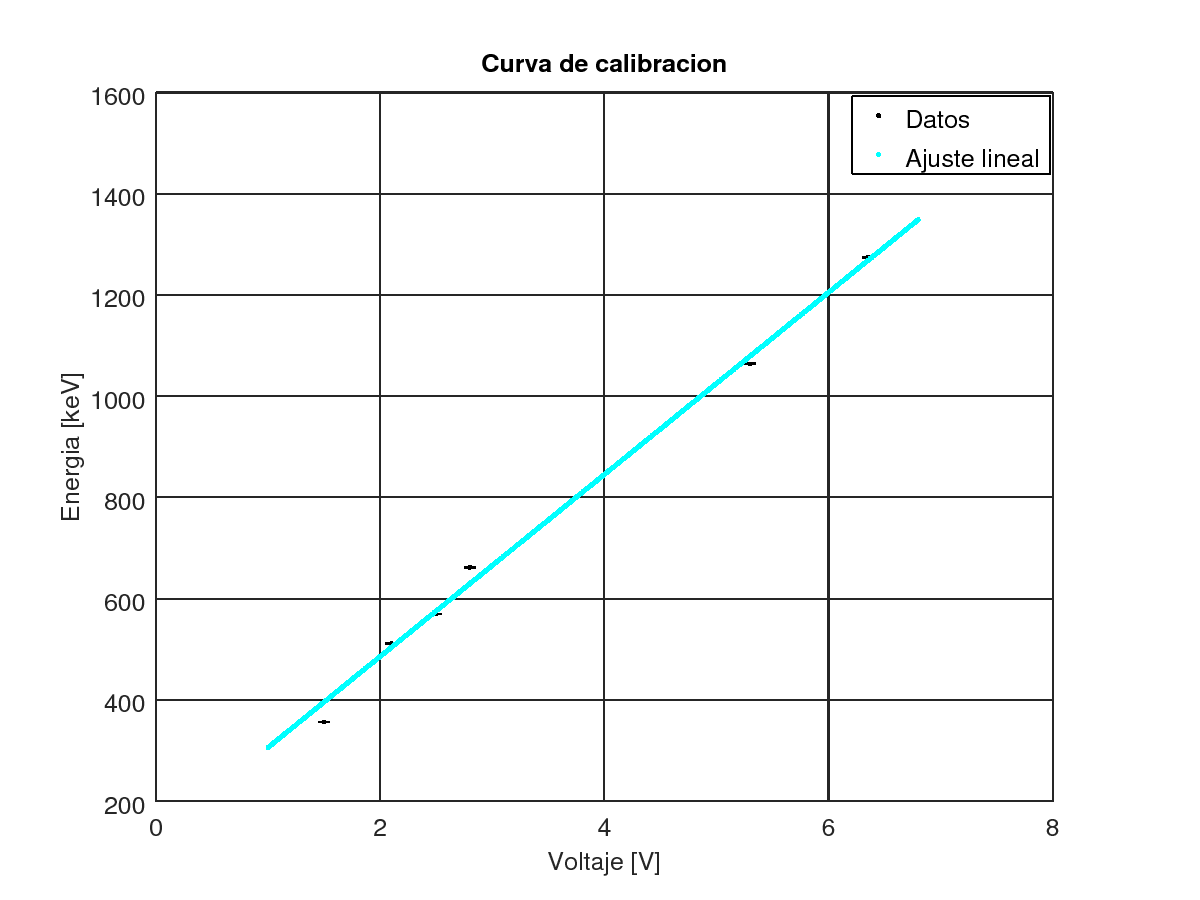
\includegraphics[scale=0.4]{calibracion1.png}
    \caption{Calibración del PMT. La relación entre voltaje medido y energía incidente es lineal ($R^2$ = 0.9943).}
    \label{experimental}
\end{figure}

Una vez realizada la calibración, se estudió si existía la posibilidad de modelar satisfactoriamente el espectro del $^{137}$Cs. A tal fin, inicialmente se modelaron el borde Compton y el fotopico por separado, y luego se utilizó una función única, suma de las dos. En una situación ideal, el fenómeno Compton toma la forma de un escalón, con el borde en el vértice. En la realidad, los procesos de medición, la superposición de efectos y las limitaciones a nivel de frecuencia de muestreo y tiempos de adquisición, además de ruido, inducen a que la forma se desdibuje, haciendo, en ocasiones, difícil incluso afirmar que el fenómeno haya ocurrido (Fig.\ref{sodio}). 

En primer lugar, se hizo la aproximación de trabajar con un histograma suavizado, para tener una única <<franja>> de puntos. Se utilizó una función del software Octave que realizaba un promedio cada 15 puntos moviéndose en el eje de voltaje. La meseta Compton se modeló utilizando una sigmoide de Boltzmann, de forma
\begin{equation}
    f(x) = h - \frac{h}{1 + e^{\frac{x - a}{4b}}},
\end{equation}
con $h$ la diferencia entre el máximo y el mínimo de la curva, $a$ la distancia (en términos de la abscisa) desde el primer punto de la curva hasta el punto medio de la caída y $b$ el ancho horizontal de la caída de la curva (la región de la aceleración). Con esta función, los resultados fueron satisfactorios. Luego, se realizó nuevamente el ajuste de los fotopicos con una gaussiana del lado derecho del máximo, como descrito previamente. Con este método, el centroide del fotopico estaba ubicado en $(2.01 \pm 0.28)$V. 

A continuación, se modeló el espectro con la función suma de las dos anteriores:
\begin{equation}
    f(x) = \alpha  \left ( h - \frac{h}{1 + e^{\frac{x - a}{4b}}} \right) + \beta \left(c + A e^{-\frac{(x - \mu)^2}{2\sigma^2}} \right),
\end{equation}
con $\alpha$ y $\beta$ dos constantes de proporcionalidad. A este punto, se decidió ajustar de dos formas: dejando los nueve parámetros libres y dejando libres solo las constantes $\alpha$, $\beta$ y $A$. En ambos casos, las condiciones iniciales fueron los valores obtenidos de los ajustes por separado. Tal como cabía esperar, al liberar todos los parámetros de ajuste, el modelo representó en su totalidad a los datos (Fig. \ref{ajustelindo}). Con seis constantes fijas, el modelo fue capaz de reproducir la forma de la gaussiana, pero la meseta Compton y el valle entre el borde y el fotopico solo parcialmente: si bien se mantuvo un perfil aproximado, las intensidades no (Fig. \ref{ajustefeo}). Más allá de la bondad de cada ajuste, la Fig. \ref{ajustefeo} confirma que efectivamente la meseta Compton influye en la posición del fotopico, y que la estrategia de hallar el centroide ajustando la mitad derecha de la campana fue acertada. Entre un modelo y otro, hay un corrimiento promedio de 0.7V hacia la izquierda en la posición del centroide. 

\bigskip
\bigskip
\bigskip


\iffalse
Por ser el proceso de absorción de radiación una proceso estocástico con una probabilidad de interacción pequeña pero aproximadamente constante para un dado espesor infinitesimal de material ${\Delta}$x, esto, la cantidad de fotones ${\Delta}$N absorbidos o dispersados por la lamina de material es proporcional al numero de fotones iniciales y y el espesor infinitesimal ${\Delta}$x.
\begin{equation}
    \Delta N \approx N \cdot \Delta x
\end{equation}
Para encontrar la relación, definimos el coeficiente de atenuación lineal ${\mu _l}$ como la constante de proporcionalidad. El coeficiente de atenuación lineal ${\mu _l}$ mide la eficiencia de un material dado para absorber la radiación, y tiende a ser mayor para sustancias con alto numero atómico. Nótese ademas que ${\Delta}$N es intrínsecamente negativo dado que el numero de fotones decrece debido a la absorción.
\begin{equation}
    \Delta N = -\mu N \cdot \Delta x
\end{equation}
Si ahora consideramos que la substancia absorbente esta separada en m capas, el numero remanente de fotones luego de atravesar completamente la substancia absorbente es ${N _m}$ = ${{N _0 \cdot \left(1 - \mu \Delta x \right)}^m }$ , si el espesor total de la substancia absorbente es L , ${\Delta x = \frac{L}{m}}$.
\begin{equation}
	{N _m = N _0 \cdot \left(1 - \mu \frac{L}{m} \right)}^m
\end{equation}
Realizando ahora un paso al limite obtenemos la expresión que rige la absorción de radiación en la materia :
\begin{equation}
	N = \lim_{m\rightarrow\infty} N_m = \lim_{m\rightarrow\infty} {N _0 \cdot \left(1 - \mu \frac{L}{m} \right)}^m = N_0 \cdot e^{-\mu _l L}
\end{equation}

donde ${N_0}$ es el numero incidente de fotones gamma y N es el numero de fotones remanentes luego de atravesar una substancia de espesor L.
\fi


Al analizar el número de eventos detectados por el PMT se encontraron tres dificultades. En primer lugar, debido a que la velocidad de muestreo de la placa adquisidora de datos es menor al ancho de banda de los pulsos a la salida del amplificador, la variación en la altura de los pulsos detectados se tradujo en la presencia de cierto nivel de ruido de naturaleza estadística en el espectro. En segundo lugar, el fenómeno de absorción fotoeléctrica dentro del centellador introduce una desviación lineal en el espectro que, si no se toma en cuenta, produce una pequeña desviación en los centroides de las pulsos gaussianos del fotopico. En tercer lugar, debido tanto a la naturaleza estocástica del proceso de decaimiento radioactivo como a los procesos físicos en el interior del PMT, el pulso obtenido al hacer el análisis espectral no es una delta de Dirac, sino que que tiene una distribución de tipo gaussiana. 

\begin{figure}[H]
    \centering
    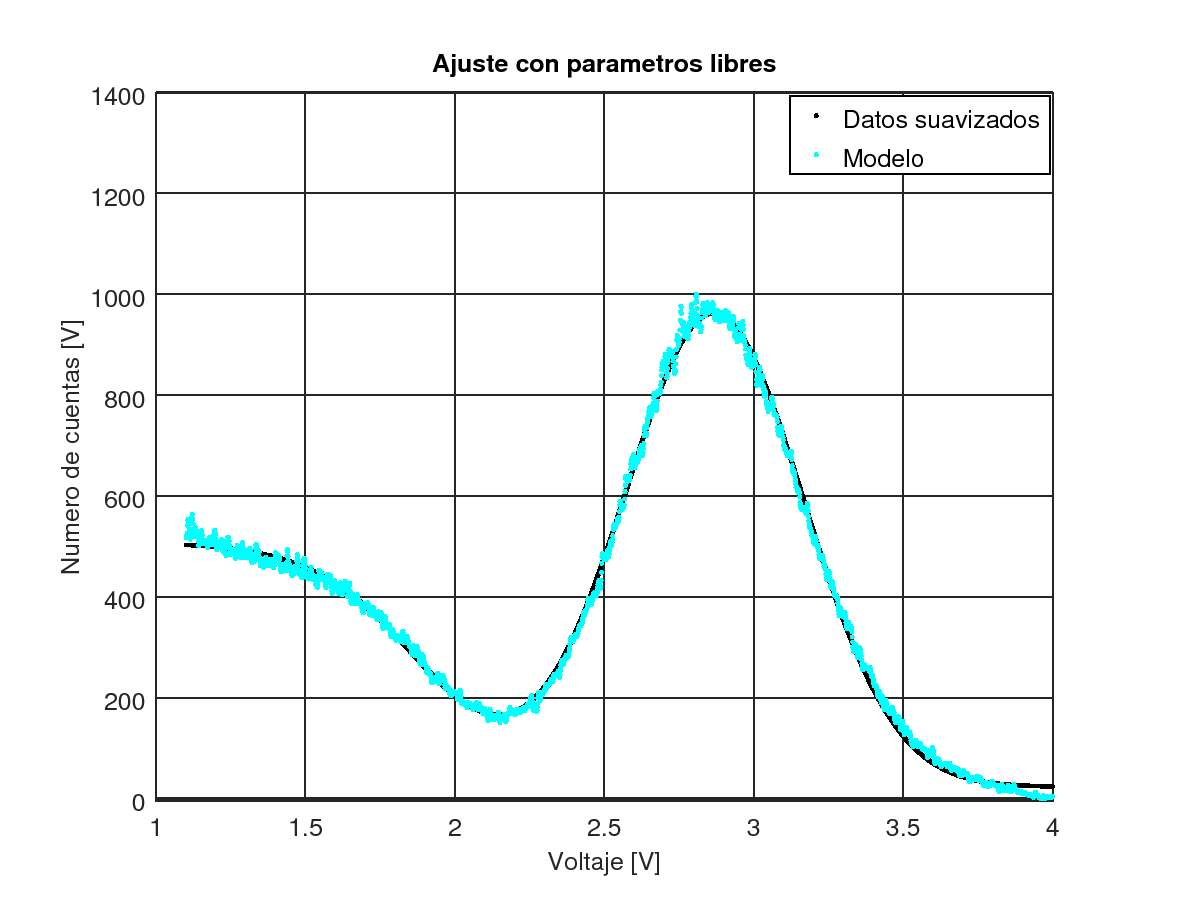
\includegraphics[scale=0.4]{ajustelindo.png}
    \caption{Ajuste del espectro con nueve parámetros libres.}
    \label{ajustelindo}
\end{figure}


\begin{figure}[H]
    \centering
    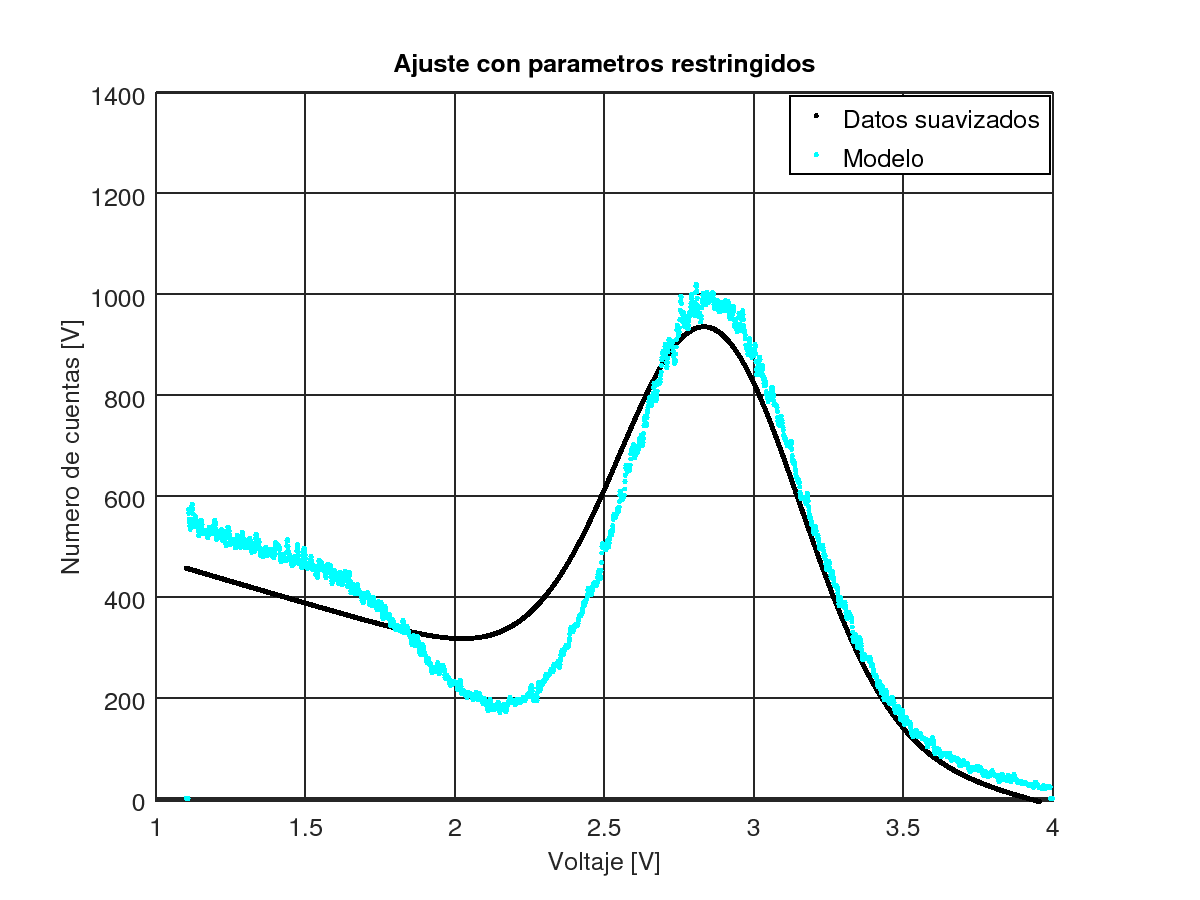
\includegraphics[scale=0.4]{ajustefeo.png}
    \caption{Ajuste del espectro con tres parámetros libres.}
    \label{ajustefeo}
\end{figure}


La primera dificultad se resolvió aplicando un suavizado a los datos utilizando un filtro de Savitzky-Golay\cite{Savitzky-Golay}. Este algoritmo realiza un ajuste por cuadrados mínimos con un polinomio de orden n alrededor de un punto ${x_0}$, utilizando n datos muestrales a cada lado del punto a suavizar. Para el set de espectros medidos se obtuvo un suavizado satisfactorio utilizado un filtro de Savitzky-Golay con un polinomio de grado 3 y 15 datos muestrales a cada lado.

Para la segunda dificultad se tuvo en cuenta que la curva de absorción fotoeléctrica con la energía del cristal centellador es aproximadamente lineal en el rango de energía cercano al fotopico del ${^{137}}$Cs. Se hizo un ajuste lineal de esta curva, con el método de cuadrados mínimos, entre 518.3 keV y 841.9 keV. Luego, se restaron al espectro suavizado los valores obtenidos para eliminar, así, la influencia de este fondo sobre la posición de los centroides del fotopico.

Por ultimo, sobre los datos suavizados y corregidos, se realizó un ajuste no lineal por cuadrados mínimos utilizando un modelo gaussiano. Esto permitió aproximar, con bastante fidelidad, la forma y altura del fotopico. Para obtener el número total de cuentas N para cada fotopico, se hizo una sumatoria de todos los eventos registrados bajo la campana. Si bien no se utilizó para este experimento, otra metodología que resulta satisfactoria para este tipo de análisis consiste en calcular el valor medio del número de cuentas registradas bajo el pulso gaussiano. Puesto que el error en el conteo de eventos está determinado principalmente por la dispersión en el ancho del pulso gaussiano debido al detector, se tomó como cota máxima del error el producto del número total de cuentas por la resolución máxima del detector en el ancho total a mitad de la altura máxima del pulso (FWHM). Dado que este valor es proporcional a la raiz cuadrada del valor medio de la gaussiana{\cite{Ortec-Gamma-Ray}} y que se tiene un error debido a las cuentras sustraidas debido a la correcion del fondo lineal , la cota maxima del error es, entonces, ${\delta N = \frac{N}{\sqrt{ \left\langle N \right\rangle }} \left( 1 + \Delta N {\left( \frac{\sqrt{ \left\langle N \right\rangle}}{N}  \right)}^2  \right) }$ donde ${ \Delta N}$ es el numero de cuentas que se substrajo al restar el fondo lineal del histograma. 

El valor del coeficiente lineal de atenuación se obtuvo realizando un ajuste por cuadrados mínimos del logaritmo del número de cuentas calculado $vs$ el espesor de penetración. Se encontró un valor del coeficiente lineal de atenuación ${\mu_l}$ de (0.8168 ${\pm}$ 0.0002)cm ${^{-1}}$ a 662 keV. Utilizando el valor conocido del material absorbente, es posible calcular el valor del coeficiente másico de atenuación ${\mu_m = \frac{\mu_l}{\rho}}$, donde ${\rho}$ es la densidad medida de dicho material. El valor es, entonces, (0.0785 ${\pm}$ 0.0002) ${\frac{cm^2}{g}}$ a 662 keV. La magnitud del coeficiente másico de atenuación está dentro de los valores esperados para diversas aleaciones reportadas\cite{bronce}, como latón (0.072 ${\frac{cm^2}{gr}}$) y bronce (0.076 ${\frac{cm^2}{gr}}$), para 662 keV.
 \begin{figure}[H]
    \centering
    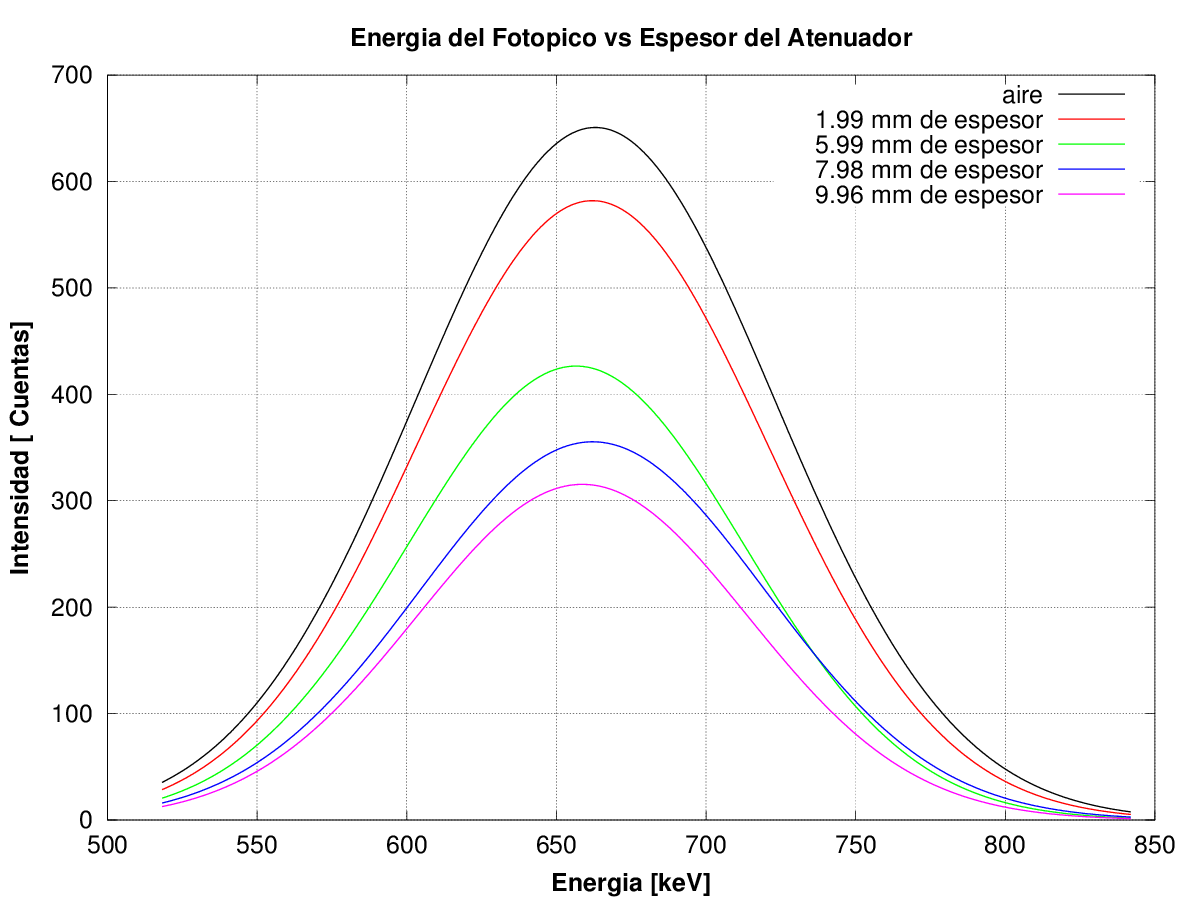
\includegraphics[scale=0.35]{Curvas_Gaussianas_Ajustadas.png}
    \caption{Curvas Gaussianas ajustadas correspondientes a cada espesor total de penetración .}
    \label{ajuste_atenuacion}
\end{figure} 



\section*{\underline{Conclusiones}}
En este trabajo se presentaron los resultados y el análisis de las experiencias realizadas con radiación gamma. En líneas generales, si bien se considera que los resultados fueron aceptables, para una próxima experiencia se recomienda el uso de detectores con mayor resolución temporal.

\begin{figure}[H]
    \centering
    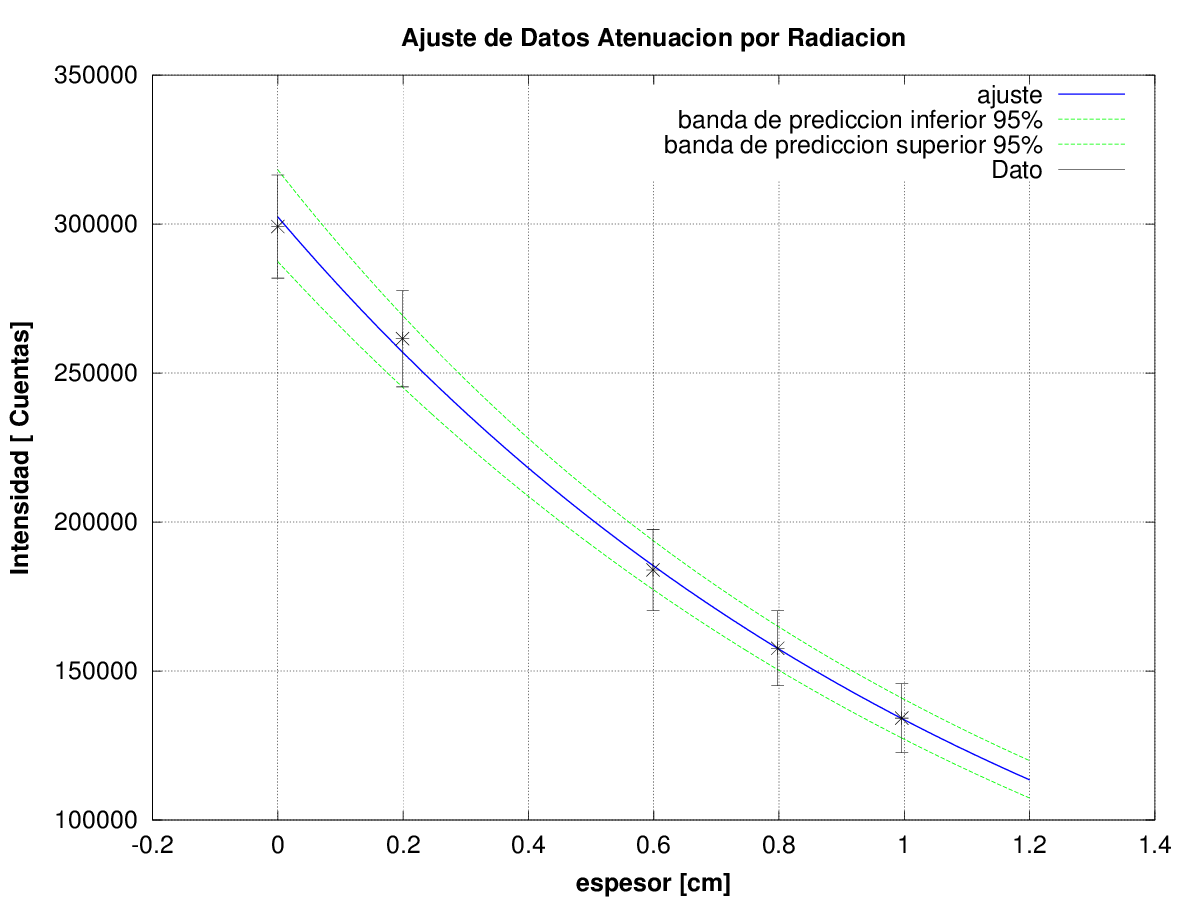
\includegraphics[scale=0.35]{Ajuste_Curva_Coeficiente_de_Atenuacion_Lineal.png}
    \caption{Se observa del ajuste una buena concordancia con el carácter exponencial decreciente de la atenuación de la  con el espesor del material absorbente.}
    \label{ajuste_atenuacion}
\end{figure}

Se modeló el espectro completo del $^{137}$Cs con una función que era combinación de una sigmoide de Boltzmann y una gaussiana. Al liberar todos sus parámetros, se obtuvo un ajuste excelente; al restringirle seis de nueve, el modelo ya no fue capaz de representar a los datos en su totalidad. Sin embargo, de este estudio se pudo confirmar que la presencia del efecto Compton afectaba la posición del fotopico, desplazándolo ligeramente hacia la izquierda.

Durante el estudio de la atenuación de la radiación con la distancia y la materia también se pudo apreciar un corrimiento hacia la izquierda a medida que se aumentaba la cantidad de láminas entre el detector y la fuente. Al momento de hallar los coeficientes de atenuación lineal (${\mu_l}$ de (0.8168 ${\pm}$ 0.0002)cm ${^{-1}}$) y másico ($\mu_m = (0.0785 \pm 0.0002)$cm$^2$/g) se notó la influencia de las incertezas experimentales, y una hipótesis que se tiene es que las láminas podrían no haber sido de cobre puro (algo que se tomó como suposición inicial). En una experiencia futura sería recomendable verificar este aspecto previamente.

\begin{thebibliography}{90}
\bibitem{Nelson}{G. Nelson and D. Reilly, \textit{Gamma-Ray Interacions with Matter}, chapter 2, \url{www.lanl.gov/orgs/n/n1/panda/00326397.pdf}}
\bibitem{poisson}{AA. VV., \textit{Naturaleza estadística del decaimiento radioactivo}, \url{http://users.df.uba.ar/bragas/Labo5_1er2011/Decaimiento.pdf}}

\bibitem{Savitzky-Golay}{A. Savitzky and M. J. E. Golay, \textit{Smoothing and differentiation of data by simplified least squares
procedures}, Anal. Chem., vol. 36, pp. 1627–1639, 1964.}
\bibitem{Ortec-Gamma-Ray}{\textit{Gamma-Ray Spectroscopy Using NaI(Ti)}, \url{ http://www.ortec-online.com/-/media/ametekortec/third\%20edition\%20experiments/gamma-ray-spectroscopy-using-nai-tl.pdf }}
\bibitem{bronce}{El-Kateb, A.H., Rizk, R.A.M., Abdul-Kader, \textit{Determination of atomic cross-sections and effective atomic numbers for some alloys}, A.M. 2000, Ann. of Nuc. Ene. 27, 1333 }
\end{thebibliography}

\end{multicols}

\end{document}



